\documentclass[11pt,letter, swedish, english
]{article}
\pdfoutput=1

\usepackage{../custom_as}
\usepackage[makeroom
]{cancel}
\graphicspath{{figures/}}


\swapcommands{\Omega}{\varOmega}

%%Drar in tabell och figurtexter
\usepackage[margin=10 pt]{caption}
%%För att lägga in 'att göra'-noteringar i texten
\usepackage{todonotes} %\todo{...}

%%För att själv bestämma marginalerna. 
\usepackage[
%            top    = 2.5cm,
%            bottom = 3cm,
%            left   = 3cm, right  = 3cm
]{geometry}

%%För att ändra hur rubrikerna ska formateras


%\renewcommand{\thefootnote}{\fnsymbol{footnote}}

\renewcommand{\thesubsection}{\arabic{section} (\alph{subsection})}
\renewcommand{\thesubsubsection}{\arabic{section} (\alph{subsection},\,\roman{subsubsection})}


\begin{document}




%%%%%%%%%%%%%%%%% vvv Inbyggd titelsida vvv %%%%%%%%%%%%%%%%%

\title{Numerical solutions to PDE's -- AMATH\,741 \\
Assignment 1}
\author{Andréas Sundström}
\date{\today}

\maketitle

%%%%%%%%%%%%%%%%% ^^^ Inbyggd titelsida ^^^ %%%%%%%%%%%%%%%%%

\section{Advection-diffusion equation}

Here we will consider the equation
\begin{equation}\label{eq:1_start}
u_t+au_x=\sigma u_{xx}\qcomma
a>0\qcomma \sigma>0
\end{equation}
on some domain.
The solutions are assumed to be of the form
\begin{equation}\label{eq:1_sol1}
u(x, t)=\sum_k \hat{u}(k, t)\ee^{\ii kx}.
\end{equation}
(The exact specification of $k$ in the sum is not given here. That is
because the values of $k$ depends on the IC or BC.)

\subsection{Finding a solution}
To find the form of each term in \eqref{eq:1_sol1}, we can omit the
sum in \eqref{eq:1_sol1}, since the governing PDE is linear. We get
\begin{equation}\label{eq:1_disp}
\hat{u}_t + \ii ka\, \hat{u}
=-\sigma k^2\hat{u},
\end{equation}
where we've also canceled the factor $ee^{\ii kx}$ appearing in all of
the terms in the dispersion relation \eqref{eq:1_disp}. We see now
that \eqref{eq:1_disp} is a DE in $t$ with the solution
\begin{equation}
\hat{u}(k, t)= c(k)\, \ee^{-(\ii ka+\sigma k^2)t},
\end{equation}
where $c(k)$ is some function of $k$ (that depends on the I.C.).
The solution to \eqref{eq:1_start} thus becomes
\begin{equation}\label{eq:1_sol2}
u(x, t) = \sum_k c(k)\, \ee^{\ii k(x-at)}\ee^{-\sigma k^2t}.
\end{equation}

The initial conditions come into play on determining $c(k)$. Let's say
that
\begin{equation}
u(x, 0)=\varphi(x)
\end{equation}
on the domain of the problem. Then, setting $t=0$ in
\eqref{eq:1_sol2}, we get
\begin{equation}\label{eq:1_F-series}
\sum_k c(k)\, \ee^{\ii kx}=\varphi(x)
\end{equation}
This is a Fourier series expansion of $\varphi$; for this to work we
need  either of these two cases to be satisfied
\begin{enumerate}[label=\Roman*.]
\item the domain of the problem is bounded with length $P$,
\item or $\varphi$ is periodic with period $P$,
\end{enumerate}
and also that $\varphi\in\mathcal{L}^2[x_0, x_0+P]$.
The allowed frequencies will be $k=n/P$, $n\in\Z$.
And the coefficients are the regular Fourier coefficients
\begin{equation}
c(k)=\frac{1}{P}\int_{x_0}^{x_0+P} \varphi(x)\ee^{-\ii kx}\id{x}.
\end{equation}

An example of a possible IC of the first kind would be 
\begin{equation}
\varphi_\mathrm{I}(x)=1-|x|
\end{equation}
on the finite domain $x\in[-1, 1]$. An expample of the second kind of
IC could be
\begin{equation}
\varphi_\mathrm{II}(x)=\cos(x)+\cos(2x)
\end{equation}
on $x\in\R$.


\subsection{Periodic boundary conditions}
\begin{figure}\centering
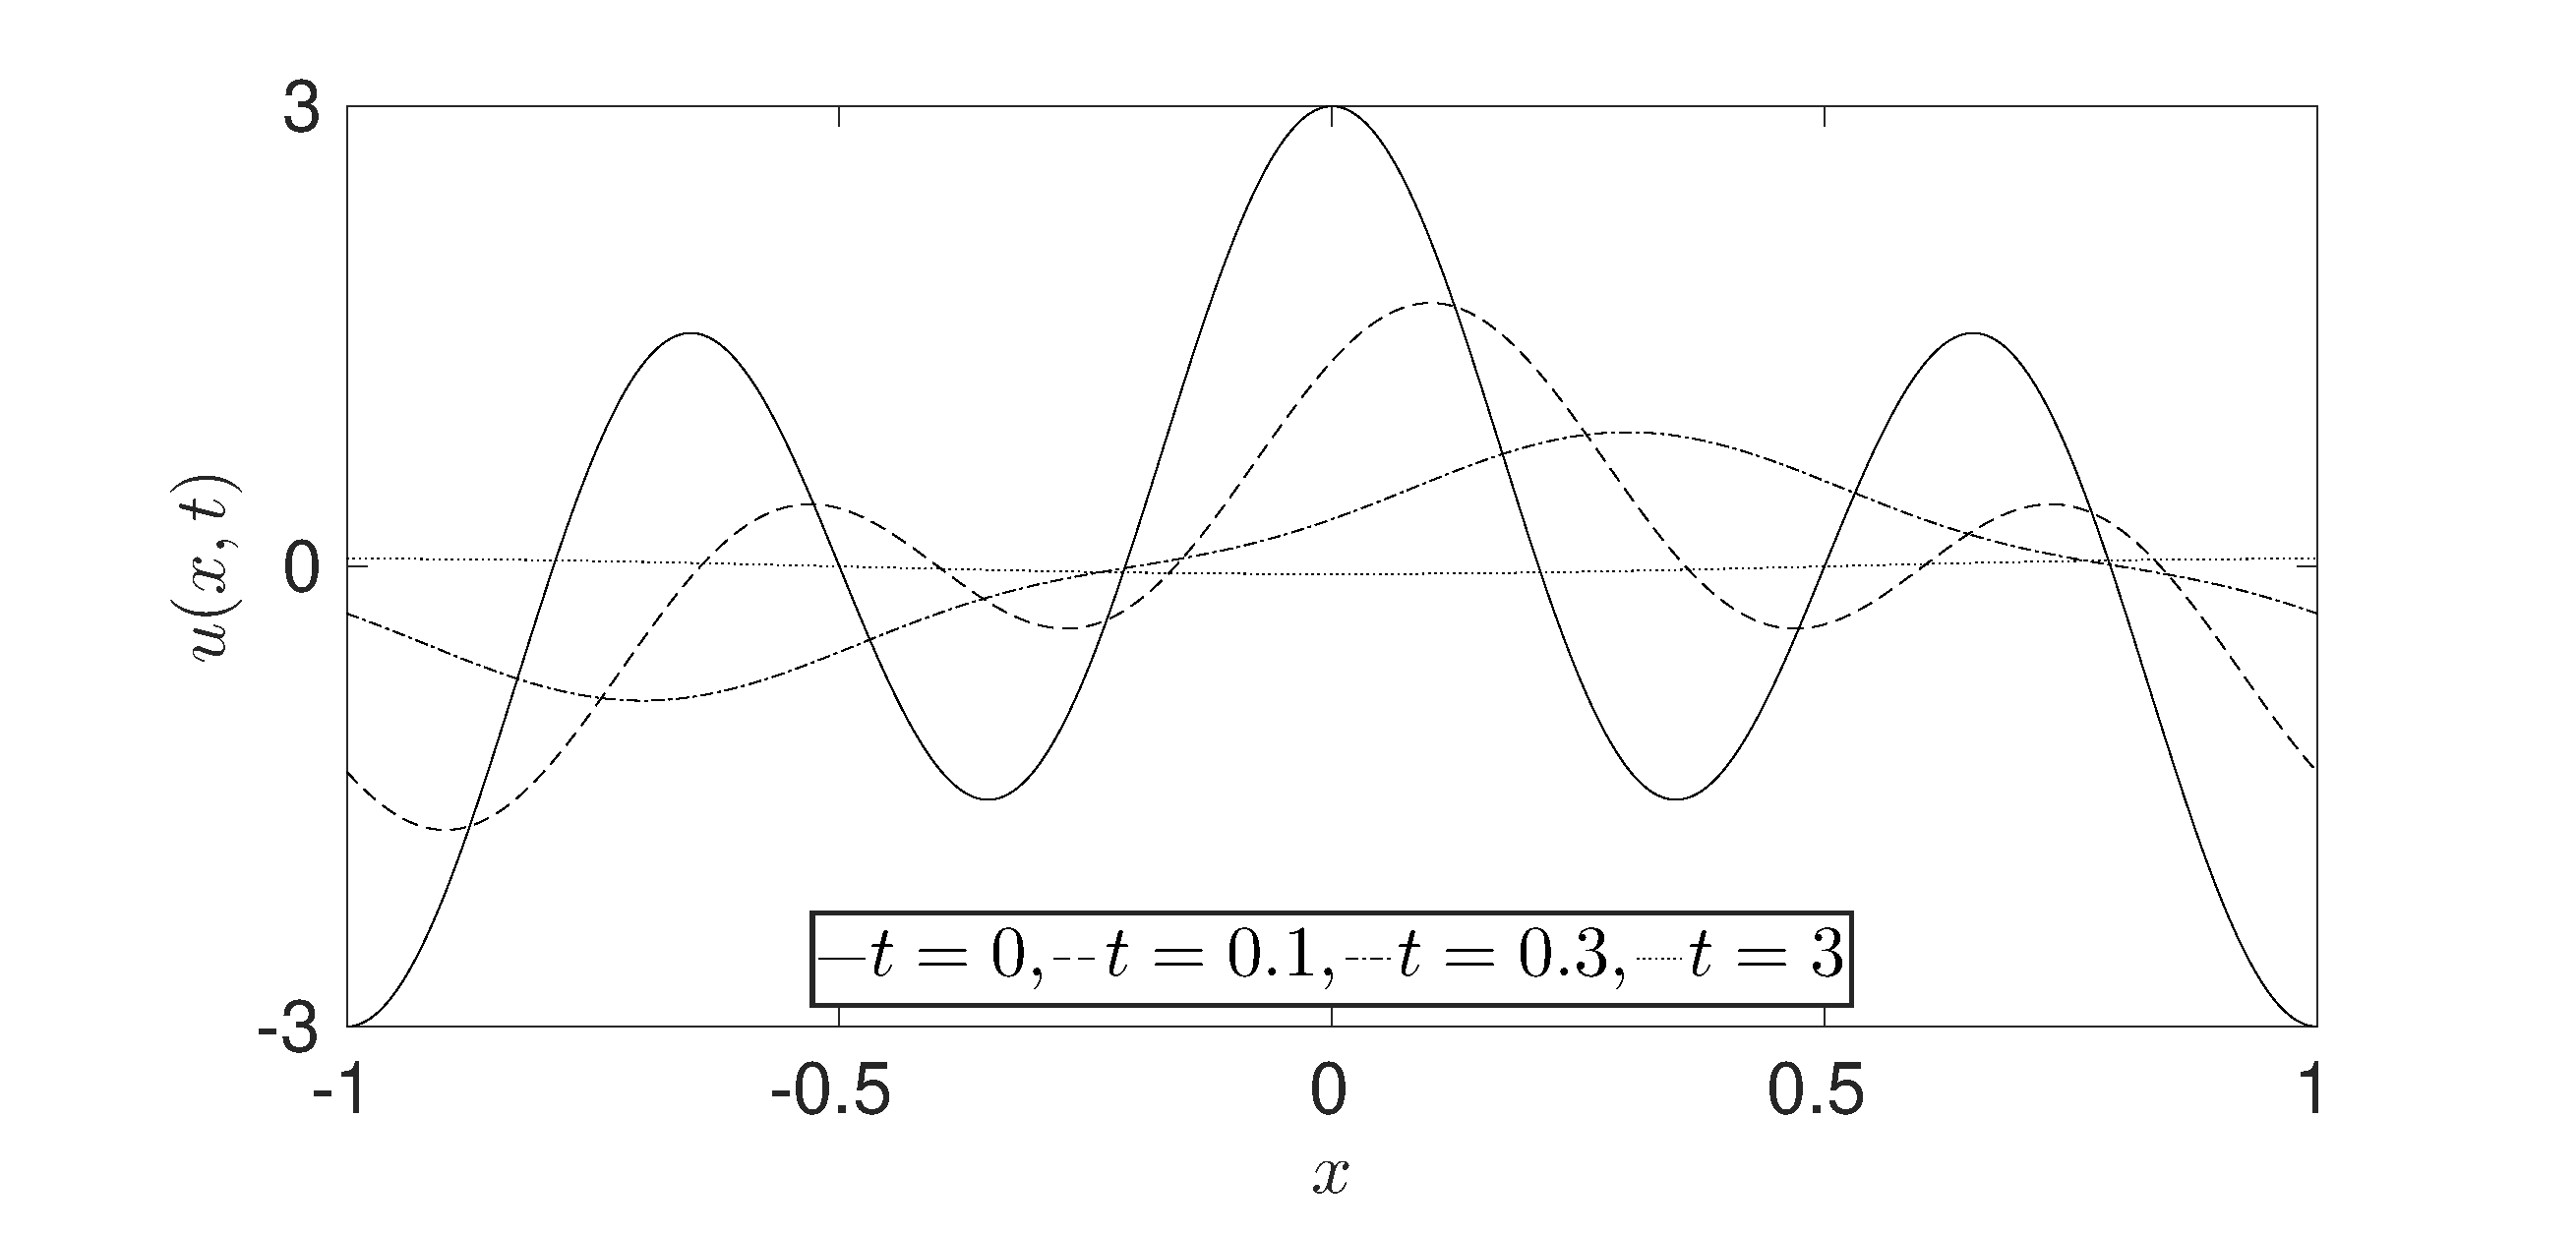
\includegraphics[width=.8\textwidth]{1_time_evolution.eps}
\caption{The time evolution of a soluotion to \eqref{eq:1_start} with
  periodic BC. The parameter values and IC are: $\sigma=a=1$ and 
  $\varphi(x)=\cos(\pi x)+2\cos(3\pi x)$. We see how, at $t=0.2$, the
  general form of the function is shifted to the right and not
  distorted very much; but at $t=0.3$ we also see that the high
  frequency component have been attenuated more; at $t=3$ almost all
  of the fluctuations are gone.}
\label{fig:1}
\end{figure}

Periodic bondary conditions are equivalent to changing from case I to
case II. 

What will happen is that each frequency will be attenuated according
to $\ee^{-\sigma k^2t}$, and then Fourier analysis tells us that the
(space domain) solution will be shifted\footnotemark{} by $at$ (to
the right for $t>0$). 

\footnotetext{See part (c) of this problem for more details.}

An exampe of this behaviour is shown in \figref{fig:1}.

\subsection{Relating this solution to the solutions of the original PDE's}
As said before the factor $\ee^{-\ii kat}$, resulting from the term
$au_x$ in \eqref{eq:1_start}, translates the solution in the positive
direction of the $x$-axis with time. To see this we have to go back to
the Fourier series \eqref{eq:1_F-series}; if we multiply the LHS by
$\ee^{-\ii kat}$ and change variables to $y=x-at$, we see that
\begin{equation}
\sum_k c(k)\, \ee^{\ii k(x-at)}=\sum_k c(k)\, \ee^{\ii ky}
\stackrel{\eqref{eq:1_F-series}}{=}\varphi(y)=\varphi(x-at).
\end{equation}
This is the behaviour expected if $\sigma=0$, i.e. when we only have
the advection equation. This is also the exact behaviour of solutions
to the advection equations. 

In the other case, where $a=0$, we see that 
\begin{equation}
u(x, t) = \sum_k c(k)\, \ee^{\ii kx}\ee^{-\sigma k^2t}.
\end{equation}
Where basically each frequency component get attenuated based on the
frequency. This is the exact behavoiur expected from a solution to the
pure heat equation. 

Together we get a mix of both. The whole solution gets shifted to the
right (due to the advection part), while each frequency component at
the same time gets attenuated (due to the heat equation part). 




\section{Higher order approximations of derivatives}
\newcommand{\Dx}{\ensuremath{\Delta{x}}}
We want to find approximations to derivatives to some reasonalby
smooth function $u$, using the functional values from points away from
the point of interest. In other words, we are looking for $C_i$ such
that\footnotemark{}
\begin{equation}\label{eq:2_start}
u_{dx}=\frac{d!}{\Dx^d} \sum_i C_i u(x+i\Dx) \quad+\order{\Dx^E},
\end{equation}
where
\begin{equation}
u_{dx}:=\pdv[d]{u}{x}
\end{equation}
is the definition of the notation, $E$ is some order of the truncation
error and the sum is some given set of $i$'s.
\footnotetext{The $t$ dependence have not been written out explicitly
  since this problem only concerns derivatives of one kind.}


We can begin by Taylor expanding $u(x+i\Dx)$:
\begin{equation}\label{eq:2_Taylor0}
u(x+i\Dx) = \sum_{n=0}^{d+E-1}
\frac{i^n\Dx^n}{n!} u_{nx}(x)
\quad+\order{\Dx^{d+E}}
\end{equation}
The expansion is done up to order $d+E-1$ because that's all we need
given the error in \eqref{eq:2_start}. Now substitute
\eqref{eq:2_Taylor0} into \eqref{eq:2_start}: 
\begin{equation}
u_{dx}=\frac{d!}{\Dx^d} \sum_{n=0}^{d+E-1}
\frac{\Dx^n}{n!} u_{nx}(x) \sum_i i^nC_i 
\quad+\order{\Dx^E}.
\end{equation}
Note that the order of the sums have been switched; this is okay since
we're only dealing with finite sums. 

Now if we disregard the error term at the end, we see that for the RHS
to be equal to the LHS $C_i$ have to be such that\footnotemark{}
\begin{equation}
\sum_i i^nC_i=
\begin{cases}
1\qcomma&n=d,\\
0,& n\neq d.
\end{cases}
\end{equation}
This is a linear system of equations 
\begin{equation}
\mathsf{A}\vb*{C}=[0, \ldots, 0, 1, 0, \ldots, 0]^\mathsfrm{T}
\end{equation}
with $I=$ ``the number of different
$i$'s'' unknowns, so we need $I$ equations; that is $I=d+E$. Basically
the number of $i$'s is determined by the order of the derivative and
how much error you want. 
Once the system of equations is solved, we get our approximation to
the derivative by plugging the $C_i$'s back into \eqref{eq:2_start}.

\footnotetext{As always with Taylor expansions, we asume the convention
that $``0^0"=1$.}

\subsection{Second and third derivative}
Here we will be using $u_j$, $u_{j\pm1}$ and $u_{j\pm2}$ to
approximate $(u_{xx})_j^n$ and $(u_{xxx})_j^n$. We see that we have
$I=5$ diffent values of $i\in\{-2, -1, 0, 1, 2\}$, so we have a
$5\times5$ system of equations with the matrix
\begin{equation}
\mathsf{A}=
\begin{bmatrix*}[r]
1&1&1&1&1\\
-2&-1&0&1&2\\
4&1&0&1&4\\
-8&-1&0&1&8\\
16&1&0&1&16
\end{bmatrix*}.
\end{equation}

For the second derivative we have
\begin{equation}
\mathsf{A}\vb*{C}=[0, 0, 1, 0, 0]^\mathsfrm{T},
\end{equation}
which has the solution
\begin{equation}
\vb*{C}=\frac{1}{24}[-1, 16, -30, 16, -1]^\mathsfrm{T}.
\end{equation}
When plugged back into \eqref{eq:2_start}, we get
\begin{equation}
(u_{xx})_j^n=\frac{-u_{j+2}^n+16u_{j+1}^n-30u_{j}^n+16u_{j-1}^n-u_{j-2}^n}{12\Dx^2}
+\order{\Dx^4}.
\end{equation}
Note that according to the prescription $I=d+E$ we should have gotten
$\order{\Dx^3}$ as the error, but due to the symmetry in the Taylor
expansion the $\Dx^3$ term vanishes. 

For the third derivative we get
\begin{equation}
\mathsf{A}\vb*{C}=[0, 0, 0, 1, 0]^\mathsfrm{T},
\end{equation}
which has the solution
\begin{equation}
\vb*{C}=\frac{1}{12} [-1, 2, 0, -2, 1]^\mathsfrm{T}.
\end{equation}
When plugged back into \eqref{eq:2_start}, we get
\begin{equation}
(u_{xxx})_j^n=\frac{-u_{j+2}^n+2u_{j+1}^n-2u_{j-1}^n+u_{j-2}^n}{2\Dx^3}
+\order{\Dx^2}.
\end{equation}

\subsection{Fourth forward derivative}
The method presented in the begining of this problem is general. All
we need to do is to pick what error we want, and then we know how many
steps we need. The only thing to keep in mind is that we're looking
for a \emph{forward} derivative, whic means that we can oly choose
$i\ge 1$.

Let's say we want an error of $E=2$, then $I=d+E=6$, so we choose
$i\in\mathcal{I}=\{0, 1, 2, 3, 4, 5\}$. The matrix elements are 
\begin{equation}
\mathsf{A}_{mn}=m^{n}
\qcomma m\in\mathcal{I}\qcomma n\in\mathcal{I}.
\end{equation}
And the matrix equation is
\begin{equation}
\mathsf{A}\vb*{C}=[0, 0, 0, 0, 1, 0]^\mathsf{T},
\end{equation}
which has the solution
\begin{equation}
\vb*{C}=\frac{1}{24} [3, -14, 26, -24, 11, -2]^\mathsf{T}.
\end{equation}
And substituting that back into \eqref{eq:2_start} yields
\begin{equation}
(u_{4x})_j^n=\frac{3u_{j}^n-14u_{j+1}^n+26u_{j+2}^n-24u_{j+3}^n+11u_{j+4}^n-2u_{j+5}^n}{\Dx^4}
+\order{\Dx^2}.
\end{equation}


\section{Round-off errors}
Here we're going to study round-off errors.

\begin{figure}\centering
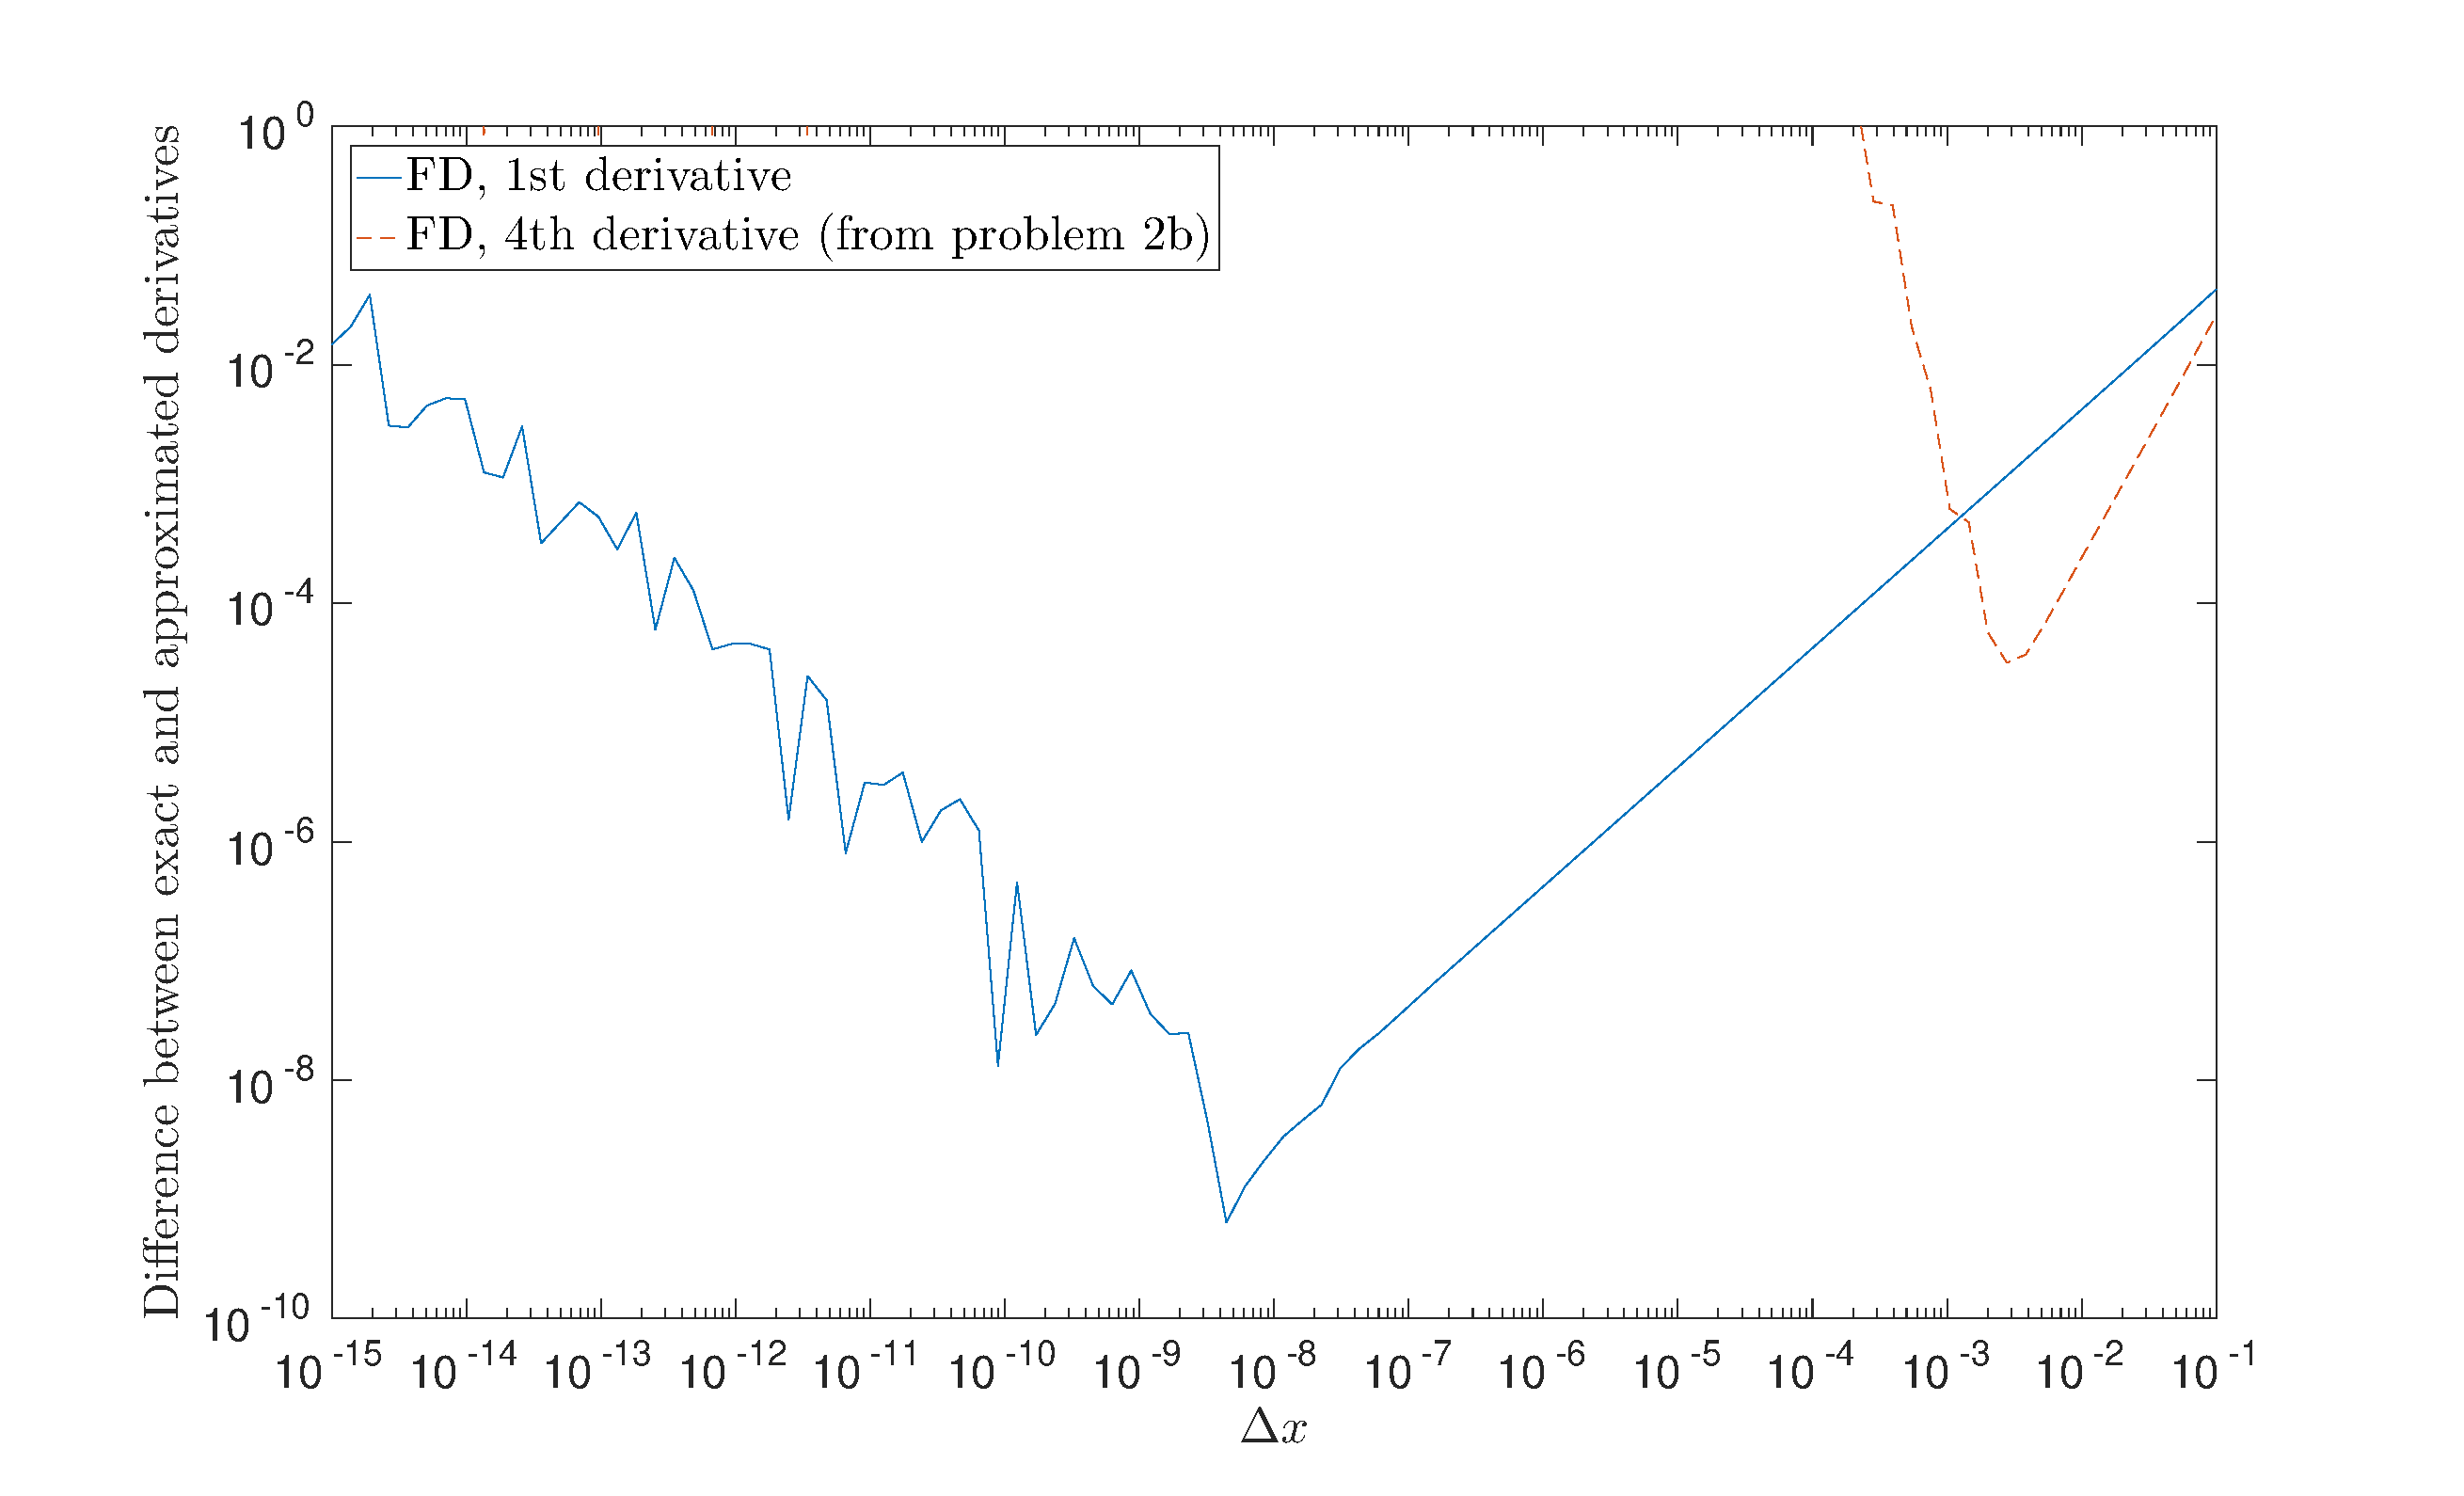
\includegraphics[width=1\textwidth]{3_FD.eps}
\caption{}
\label{fig:3_error}
\end{figure}



\section{Numerical solution of the heat equation}







\end{document}




%  LocalWords:  MFT MF Advection PDE's AMATH
